\documentclass[a4paper,10pt]{article}


\usepackage[spanish]{babel}
\usepackage[utf8]{inputenc}


\usepackage{amsmath, amsfonts}
\usepackage{graphicx}
\usepackage{natbib}
\usepackage{caption}
\usepackage{subcaption}



\bibliographystyle{alpha}

%opening
\title{Cálculo detallado del volumen de un cilindro con cuñas en cuatro
Dimensiones}
\author{Rosa Rodríguez \& David P.~Sanders \& W. P. K. Zapfe}
%\address{Departamento de Física, Facultad de Ciencias, Universidad Nacional Autónoma de México, Ciudad Universitaria, Del.~Coyoacán, México D.F. 04510, Mexico}

\usepackage{mathptmx}

\newcommand{\defeq}{:=}
\newcommand{\mean}[1]{\left \langle #1 \right \rangle}
\newcommand{\rd}{\, \mathrm{d}}
\newcommand{\RR}{\mathbb{R}}
\newcommand{\vv}{\mathbf{v}}
\newcommand{\indicator}[1]{\mathbf{1}_{ \{   #1 \} } } 
\newcommand{\Indi}{\mathbf{1}}


\setlength{\parskip}{10pt}
\setlength{\parindent}{0pt}

\begin{document}

\maketitle

\section{Volumen}

Vamos a detallar como  se obtiene el volumen de un cilindro
encajado en un hipercubo de forma diagonal, y explicar porqué el 
método ``de interpretación geométrica'' resulta en un error. 

Seguiremos las notas de Rosa Rodríguez, expandiendo los detalles
más truculentos de la integración. Nuestro volumen de integración
depende de las siguientes condiciones del sistema dinámico:

Tenemos una mesa de billar cuadrangular de lados de tamaño 
$w,h$ a lo largo de los ejes horizontal y vertical usuales
de un sistema cartesiano. Dentro de ella se mueven
discos rígidos de radio $r$ y diámetro $2r=d$.  Cada disco
tiene centro de coordenadas $(x_i, y_i), i=1,2$. Por la
estricta rigidez de los discos, sus centros se mueven
en un espacio efectivo menor a la mesa de billar. Si definimos
$a:=w/2-r$, $b:=h/2-r$, los centros cumplen con:
\begin{equation}
(x_i, y_i)\in [-a,a]\times [-b,b].
\end{equation}
Véase la figura \ref{Billar01}

\begin{figure}[h]
  \centering
  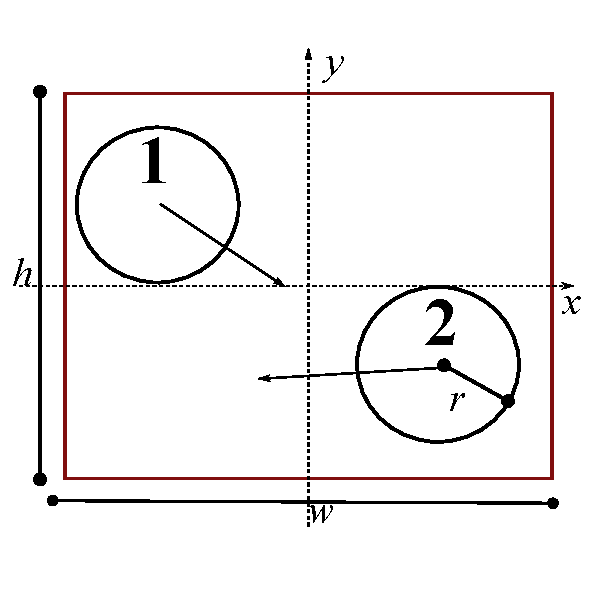
\includegraphics[width=0.56\textwidth]{DiscosenCajaCuadrada01.pdf}
  \caption{El Billar}\label{Billar01}
\end{figure}

El choque ocurre \emph{exactamente} cuando los discos se tocan,
es decir, cuando sus centros se encuentran a distancia $d$. 
\begin{equation}\label{condencuentro}
(x_1-x_2)^2+(y_1-y_2)^2=d^2.
\end{equation}
La exclusión del espacio de configuraciones total
viene dada por todos los puntos $(x_1,x_2,y_1,y_2)$ cuyas
coordenadas cumplan con:
\begin{equation}
(x_1-x_2)^2+(y_1-y_2)^2<d^2.
\end{equation}
Esto es el volumen prohibido en el espacio de configuraciones
total, que es un hipercubo de lados $2a,2a, 2b, 2b$. 

Calculemos, pués, el volumen prohibido y encontremos que restándoselo
al volumen del hipercubo, obtenemos lo mismo que Munakata y Hu. 

Llevamos a cabo la siguiente transformación isométrica de coordendadas:
\begin{align}
x &:=\frac{x_1-x_2}{\sqrt{2}}, & X &:=\frac{x_1+x_2}{\sqrt{2}}, \\
y &:=\frac{y_1-y_2}{\sqrt{2}}, & Y &:=\frac{y_1+y_2}{\sqrt{2}}.
\end{align}
que hace ver más simple la condición de exclusión:
\begin{equation}\label{exclu01}
(x)^2+(y)^2<d^2/2 = 2r^2.
\end{equation}

La figura excluida es cilindro con dos ejes: $X,Y$, que se encuentran
diagonalmente insertados en el hipercubo. Las puntas del cilindro no
son ya circulares, puesto que la frontera del hipercubo las intersecta, 
esto es la condición:
\begin{equation}\label{cunha01}
|X|<a\sqrt{2}-|x|,\;  |Y|<b\sqrt{2}-|b|.
\end{equation}
Esto es más simple viendo un diagrama de producto de espacios:
el espacio de los pares \emph{horizontales} $(x_1,x_2)$ y el de los
verticales, $(y_1,y_2)$, figura \ref{ProductoEspacios01}.
\begin{figure}[h]
  \centering
  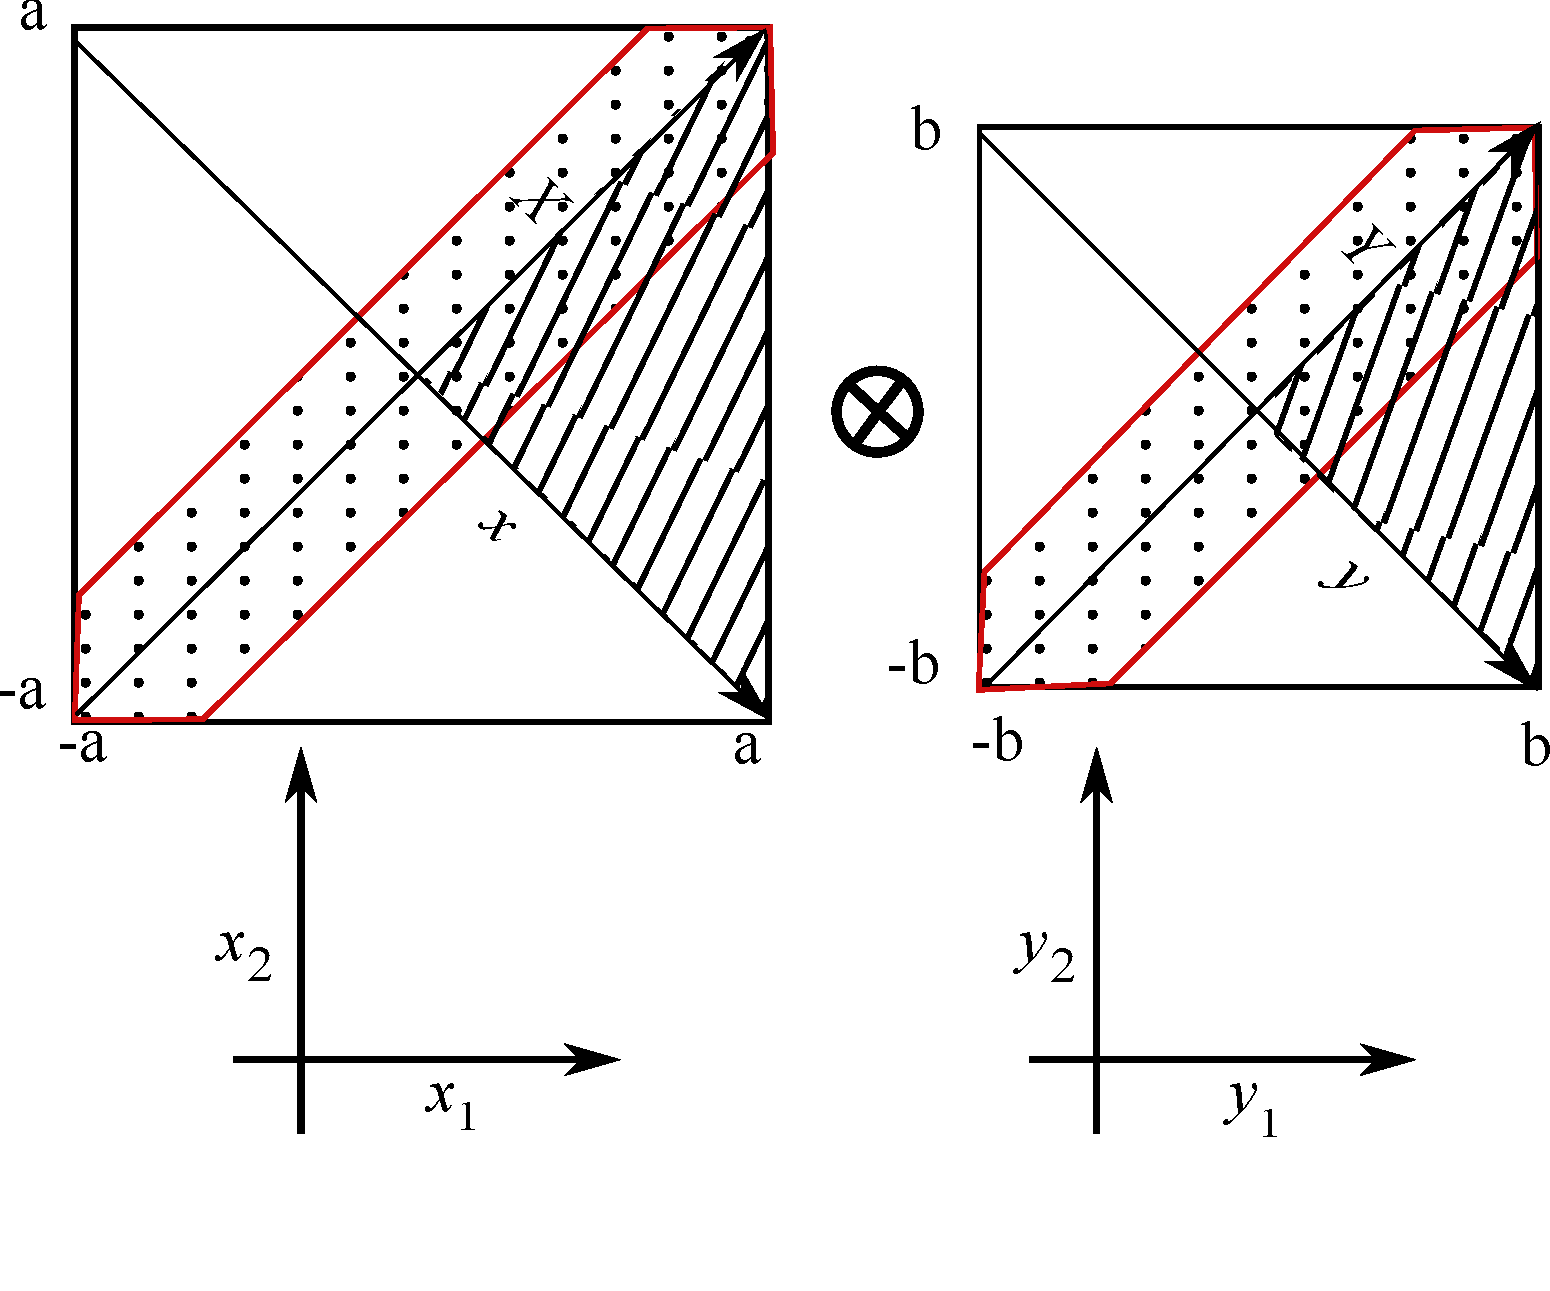
\includegraphics[width=0.56\textwidth]{diagramintegra01.pdf}
  \caption{El Producto de espacios.}\label{ProductoEspacios01}
\end{figure}

Tanto el diagrama, como los valores absolutos que aparecen
en las condiciones \ref{cunha01} y \ref{exclu01} (implicitamente),
nos hacen ver que hay una simetría cuadrangular en ambos
elementos del producto de espacios. Asi que bastará resolver
la integral en el área triangular rayada en la figura, y
multiplicar por $4\cdot 4 = 16$. Podemos escoger integrar
las áreas libres (sin color) o el área excluida (con color), y restarsela al 
hipercubo. Yo escogeré la segunda. 

El volumen está dado por la integral de la función indicatriz por el 
elemento de volumen. Hagamos esto de forma muy explicita, paso por paso:

\begin{equation}
V/16 =\iiiint \rd X \rd Y \rd x \rd y 
\Indi \{(x)^2+(y)^2<d^2/2,\; |X|<a\sqrt{2}-|x|,\;  |Y|<b\sqrt{2}-|b|\}
\end{equation}

La integral sobre $X,Y$ está dada por los límites dados por la condición
\ref{cunha}, así que despachamos esa parte funcional rápidamente en la sección rayada:

\begin{equation}\label{Volumen01}
\begin{split}
V/16 &=\iint \rd x \rd y (a\sqrt{2}-x)(b\sqrt{2}-y)
\indicator{(x)^2+(y)^2<d^2/2 }\\
&=\iint \rd x \rd y (2ab-\sqrt{2}(ay+bx)+x y)
\indicator{(x)^2+(y)^2<d^2/2 }.
\end{split}
\end{equation}
Como sólo estamos integrando en el sector de $ x,X,y,Y > 0$, basta integrar
el \emph{cuadrante positivo} del cilindro. Nótese que el caso límite
es cuando $(2a)^2+(2b)^2=d^2$, es decir, que apenas caben los dos discos en la
caja y no tienen espacio para moverse. Si $2a<d$ o $2b<d$ uno de los dos 
intercambios de posición (o ambos) están excluidos. Sin pérdida de
generalidad podemos suponer que la mesa esta orientada siempre de forma
que $a \geq b$. Los tres casos están ejemplificados en la figura 
\ref{CasosIntegra}. Ahí se muestra además que el método más simple para
llevar la integración es usar coordenadas polares en el área roja
y cartesianas en el área verde.

\begin{figure}[h]
        \centering
        \begin{subfigure}[b]{0.32\textwidth}
          \centering
          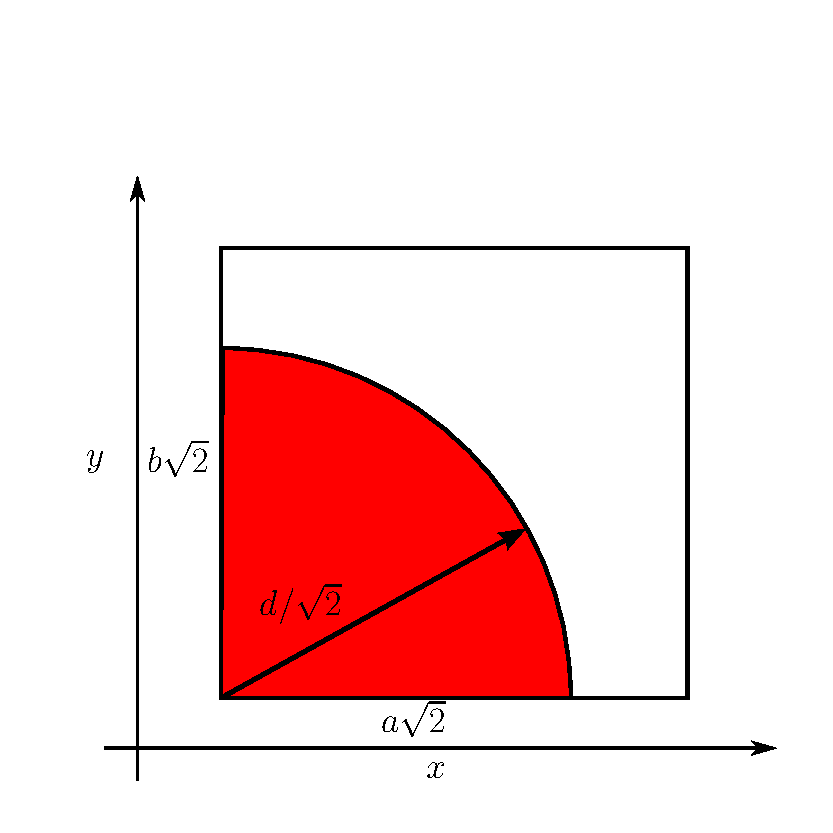
\includegraphics[width=\textwidth]{DiagramaIntegracionxy01-Bien.pdf}
          \caption{$a,b>d/2$}
          \label{smallradious}
        \end{subfigure}%
        ~ %add desired spacing between images, e. g. ~, \quad, \qquad etc.
        % (or a blank line to force the subfigure onto a new line)
        \begin{subfigure}[b]{0.32\textwidth}
          \centering
          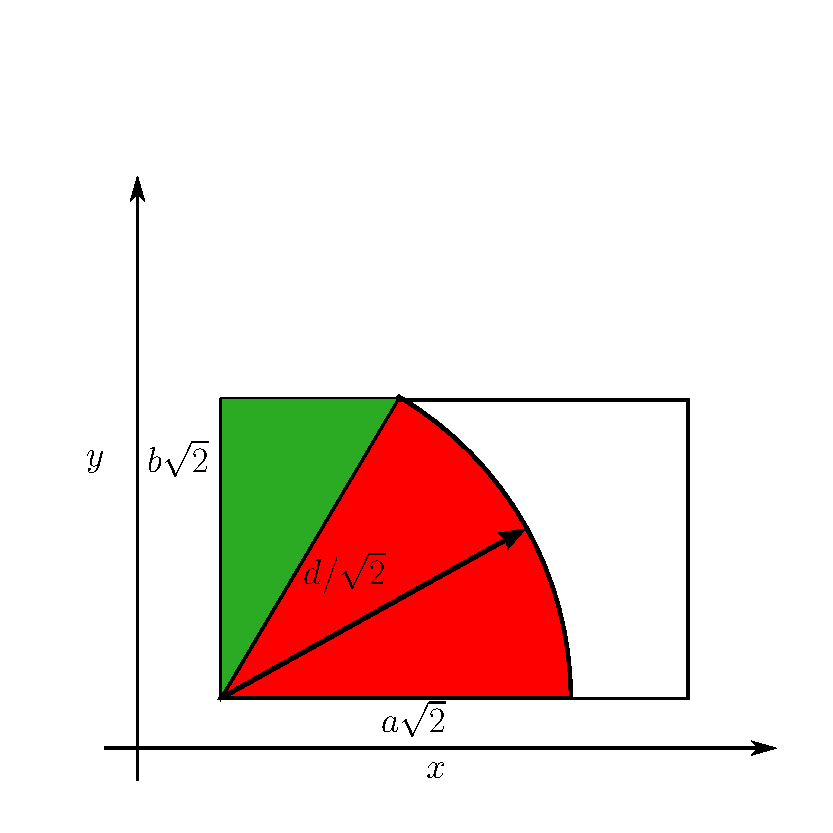
\includegraphics[width=\textwidth]{DiagramaIntegracionxy02-Bien.pdf}
          \caption{$b<d/2$}
          \label{mediumradius}
        \end{subfigure}%
        ~ %add desired spacing between images, e. g. ~, \quad, \qquad etc.
          %(or a blank line to force the subfigure onto a new line)
        \begin{subfigure}[b]{0.32\textwidth}
          \centering
          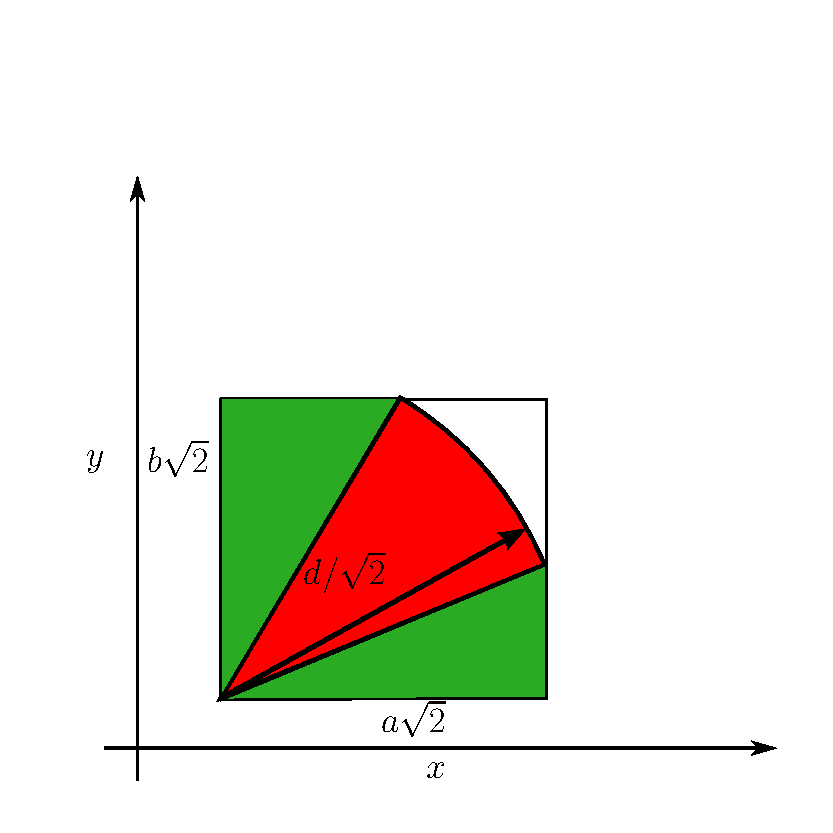
\includegraphics[width=\textwidth]{DiagramaIntegracionxy03-Bien.pdf}
          \caption{$a,b<d/2$}
          \label{bigradious}
        \end{subfigure}%
        \caption{Los tres posibles casos. En el segundo caso, un
          intercambio de posición vertical está excluido, mientras
          que en el tercero ambos intercambios de posición están excluidos.}
\label{CasosIntegra}
\end{figure}

Comencemos por el caso de la figura \ref{smallradious}. Ahí lo más simple
es usar coordenadas polares, ya que  entonces la función indicatriz simplemente
se vuelve límites de integraciónr sobre la variable radial.
\begin{equation}
\begin{split}
V/16 &=\iint \rd x \rd y (2ab-\sqrt{2}(ay+bx)+x y)
\indicator{(x)^2+(y)^2<d^2/2 }\\
&=\iint \rd \rho \rd \theta \rho (2ab
-\sqrt{2}(a\rho\sin\theta+b\rho\cos\theta)
+\rho^2 \cos\theta\sin\theta)
\indicator{\rho^2<d^2/2 }\\
&=\iint\limits_{0,0}^{\pi/2,d/\sqrt{2}} \rd \rho \rd \theta \rho (2ab
-\sqrt{2}(a\rho\sin\theta+b\rho\cos\theta)
+\rho^2 \cos\theta\sin\theta).
\end{split}
\end{equation}
Integremos de forma definida la parte radial, ya que esa se mantendrá
igual en los otros casos, mientras
 la parte angular tendrá diferentes límites. Escribamos la expresión
de forma indefinida en este caso.
\begin{equation}
\begin{split}
V/16 &=\int\limits_0^{\pi/2}  \rd \theta  
(abd^2 - d^3/6 (a\sin\theta+b*\cos\theta)+d^4/16 (\cos\theta\sin\theta))\\
&=\frac{abd^2}{2}\theta
+\frac{d^3}{6}(a\cos\theta-b\sin\theta)
-\frac{d^4}{16\cdot 4}\cos (2\theta) \bigg\vert_0^{\pi/2} \\
& =\frac{abd^2 \pi }{4}
-\frac{d^3}{6}(a+b)
+\frac{d^4}{32}.
\end{split}
\end{equation}

Finalmente multiplicamos por 16 para obtener el volumen del cilindro con
sus cuñas:
\begin{equation}\label{VolTotal}
V=4 \pi abd^2-\frac{8 d^3}{3}(a+b)+\frac{d^4}{2},
\end{equation} 
 coincidiendo con Rosa, Munakata y Hu.

Ahora bien, para generalizar a los casos mostrados en \ref{mediumradius} y 
\ref{bigradious}, tomemos primero la parte ``circular'' (roja, en los
diagramas), y evaluamos la parte angular entre los ángulos dados por las
intersecciones del área roja con el rectángulo de los diagramas.
En el caso \ref{mediumradius} esto es, 

\begin{equation}
V_{rojo} = 8abd^2\arccos(b/d)
+\frac{8 d^3}{3 }(a(b/d-1)-b(\sqrt{d^2-b^2}/d))
-\frac{d^4}{4} (2 b^2/d^2-1) 
\end{equation}

En el caso \ref{mediumradius} habría que restarle a esa expresión
la valuación en $\theta=\arccos(a/d)$, con lo que quedaría la hermosa 
expresión:
\begin{multline}
V_{rojo} = 8abd^2(\arccos(b/d)-\arccos(a/d))\\
+\frac{8 d^3}{3 }(a((b-a)/d)-b(\sqrt{d^2-b^2}/d+\sqrt{d^2-a^2}/d))\\
-\frac{d^4}{2} ( (b^2-a^2)/d^2) 
\end{multline}
La expresión es antisimétrica en $a,b$, lo cual tiene sentido ya
que recorremos el área en $\theta$ en una dirección particular.

No es tan terrible. Ahora falta por evaluar las áreas verdes. 
En ese caso es más fácil llevar a cabo la integración
en cartesianas. El tríangulo verde en la figura \ref{mediumradius}
contribuye de la forma siguiente:
\begin{equation}
\begin{split}
V_{verde}/16 & = \iint  \rd x \rd y (2ab-\sqrt{2}(ay+bx)+x y)
\indicator{\frac{xb}{\sqrt{d^2-b^2}}< y < b\sqrt{2}}\\
&=\int \rd x \bigg[ (2ab-\sqrt{2} b x) y+ y^2/2 (a \sqrt{2}+x) \bigg]
_{xb/\sqrt(d^2-b^2)}^{b\sqrt{2}} \\
&=\int \limits_0 ^{\sqrt{d^2-b^2}} \rd x 
\bigg[ab 4\sqrt{2}
-x\frac{2ab^2}{\sqrt{d^2-b^2}}
+x^2b^2\sqrt{2}(1/\sqrt{d^2-b^2}-a/(d^2-b^2))-x^3\frac{b^2}{d^2-b^2}
\bigg]
\end{split}
\end{equation}

Creo que para este momento ya debería de haber escogido un nombre
para el lado superior del rectángulo verde. Definamos
$c:=\sqrt{d^2-b^2}$.

\begin{equation}
V_{verde}=16\big( a b^2 c (4\sqrt{2}-1-\sqrt{2}/3)
+c^2b^2 (\sqrt{2}/3-1) \big).
\end{equation}

En el caso mostrado en la  figura \ref{bigradious} tendríamos
que tomar en cuenta otra contribución similar, pero con
los papeles de $a$ y $b$ invertidos. 

\section{Área}

\subsection{Área del Cilindro}

El área para el cilindro es la medida inducida por el espacio de
configuración sobre el subconjunto de puntos que satisfacen 
exactamente la condición de encuentro, que repito aquí:

\begin{equation}
(x_1-x_2)^2+(y_1-y_2)^2=d^2.
\end{equation}

Si inocententemente ponemos esta condición dentro de la función
indicatriz de la ecuación \ref{Volumen01} obtenemos cero. La forma correcta
de encontrar el área es concentrar la medida sobre la superficie
$\rho=d/sqrt{2}$. Para esto la solución es usar una delta de Dirac, lo
que equivale a concentrar la medida en una vecindad
infinitamente pequeña en la orilla del cilindro.

\begin{equation}\label{Volumen01}
\begin{split}
A/16 
&=\iint \rd x \rd y (2ab-\sqrt{2}(ay+bx)+x y)
\delta (\rho-d/\sqrt{2}) \\
&=\iint \rd \rho \rd \theta \rho (2ab
-\sqrt{2}\rho(a \cos\theta + b\sin\theta )+\rho^2 \cos\theta\sin\theta)
\delta (\rho-d/\sqrt{2})\\
&=\int\limits_{\theta_1}^{\theta_2} \rd \theta (2ab d/\sqrt{2}
-d^2/\sqrt{2}(a \cos\theta + b\sin\theta )+d^3/(2\sqrt{2}) \cos\theta\sin\theta)\\
&= \theta 2ab d/\sqrt{2}
-d^2/\sqrt{2}(a\sin\theta - b\cos\theta )-d^3/(4\sqrt{2}) \cos (2\theta) 
\bigg\vert_{\theta_1}^{\theta_2}
\end{split}
\end{equation}
Escogo dejar la integral en términos de $\theta_1$ y $\theta_2$,
así abarco los tres posibles casos, dado que las partes triangulares
no contribuyen con área accesible al punto en el espacio de configuración,
es decir, no podemos tocar esa área desde el volumen disponible.
Así que para el caso general, basta tomar los ángulos adecuados.
El caso particular donde 
$d>a,b\Rightarrow \theta_1=0, \theta_2=\pi/2$ 
da un resultado bastante coherente:
\begin{equation}\label{areachoque}
A=[8\sqrt{2}\pi ab] d -[8\sqrt{2}] (a+b) d^2 +[4 /\sqrt{2}]d^3.
\end{equation}
Podemos identificar los tres términos de forma simple:
el primero sería un hipercilindro en cuatro dimensiones, sin cuñas.
Se puede descomponer naturalmente en 
$2\pi \cdot 2a \cdot 2b \dot R$, con $R=d/\sqrt{2}$.
El segundo es el área que ocupan las cuñas, restada. El tercero,
que no depende de $a, b$, es el el área 
externa de las cuñas. La causa de  porque
los cálculos anteriores estaban mal se encuentra en el segundo término:
depende de $a,b$. Esto se debe a que la desigualdad que determina
la cuña,  $X<|x|-a\sqrt{2}$, $Y<|y|-b\sqrt{2}$ NO es independiente de
la desigualdad que determina el radio del hipercilindro, cosa que yo
desprecié en los cálculos anteriores\ldots

\subsection{Verificación por medio de la derivada respecto al Radio}

Veamos si derivando la expresión \ref{VolTotal} podemos confirmar el área 
resultante en la ec. \ref{areachoque}. Primero, debemos poner la primera
en función de un ``radio'', ya que esta evaluada así como se muestra
para un hipercilindro de radio $d/\sqrt{2}= r \sqrt{2}$. Así que escribiendo
eso para que sea evidente la valuación la fórmula cobra el siguiente aspecto:

\begin{equation}\label{VolcomoFuncion}
V(d/\sqrt{2}) =8 \pi ab (d/\sqrt{2})^2
-\frac{8 \cdot 2 \cdot \sqrt{2} (d/\sqrt{2})^3}{3}(a+b)
+\frac{4 (d/\sqrt{2})^4}{2}.
\end{equation} 

Entonces la ``función del hipervolumen'' quedará en términos de ese radio 
virtual así:

\begin{equation}\label{VolcomoFuncion}
V(x) =8 \pi ab x^2
-\frac{8 \cdot 2 \cdot \sqrt{2} x^3}{3}(a+b)
+\frac{4 x^4}{2}.
\end{equation} 

El primer término parece tener sentido, ya que las longitudes del
cilindro son $2\sqrt{2} a, 2\sqrt{2} b$, por lo tanto, el volumen
tiene la forma $\pi l_1 l_2 r^2$, como cabría de esperar. 

Considerando que el área exterior del cilindro sea la diferencial del
volumen respecto al radio, y considerando que $a,b$ no dependieran
del radio, obtenemos lo siguiente:
\begin{equation}\label{DerivadaVolcomoFuncion}
\frac{\rd V}{\rd x}(x) =8\cdot 2  \pi ab x
-8 \cdot 2 \cdot \sqrt{2} x^2(a+b)
+4 \cdot 4 / 2 x^3
\end{equation}
Valuemoslo en $x=d/\sqrt{2}$:
\begin{equation}\label{Areaconfirmada}
A(d/\sqrt{2}) =[8\cdot \sqrt{2}  \pi ab] d
-[8 \cdot  \sqrt{2} (a+b)] d^2
+ [4 / \sqrt{2}] d^3
\end{equation}
Excelente.


\subsection{Área de la sección que determina el \emph{brinco}}.

Hay dos bríncos: vertical y horizontal. Enfoquemonos en el horizontal,
que, en términos de una sección del espacio de configuración total,
ocurre cuando los dos centros de los discos se encuentran en la misma
posición. El área de esa 
sección  esta dada por la condición $x_1=x_2$, lo cual en las coordedas
sin subíndice es $x=0$.
\begin{equation}
A/8 =\iiiint \rd X \rd Y \rd x \rd y \delta(x)
\Indi \{ |X|<a\sqrt{2}-|x|,\;  |Y|<b\sqrt{2}-|b|\}
\end{equation}
Nótese que escribí $A/8$ y no $A/16$. La condición $x=0$ no tiene
dos lados, así que hay una simetría menos en el conteo de piezas.
También no especifiqué en la función indicatriz el \emph{radio}
de integración. Esto es porque es más simple llevar a cabo la 
integral en abstracto y luego tomar en cuenta el tamaño completo
de este subespacio diagonal y posteriormente descontar la parte
que corresponde al interior del cilindro. También es de 
notar que si $x=0$, la condición del interior del
cilindro queda como $y^2\leq d^2/2$, lo cual NO define una estructura
circular: en esta sección el corte del cilindro es un cubo\ldots

La integral se resuelve de forma relativamente directa.
\begin{equation}
\begin{split}
A/8 &=\iiiint \rd X \rd Y \rd x \rd y \delta(x)
\Indi \{ |X|<a\sqrt{2}-|x|,\;  |Y|<b\sqrt{2}-|b|\}\\
\iint \rd x \rd y \delta (x) (a\sqrt{2}-x)(b\sqrt{2}-y) \\
&=2aby-\frac{\sqrt{2}ay^2}{2}\bigg\vert_0^{R}
\end{split}
\end{equation}
El límite es $b\sqrt{2}$ para la sección total, y $d/\sqrt{2}$ 
para la parte que está encerrada en el cilíndro. El resultado
final, después de evaluar, sacar la diferencia y
multiplicar por ocho es:
\begin{equation}
A_{hopp}=8ab^2\sqrt{2}-8abd\sqrt{2}+2ad^2\sqrt{2}
\end{equation}
Podemos obtener el área de choque correspondiente a un brinco
vertical intercambiando los papeles de $a,b$.
Para verificar, buscamos hacer que esa área se anule 
manipulando el tamaño del diámetro $d$:
\begin{equation}
A_{hopp}=8ab^2\sqrt{2}-8abd\sqrt{2}+2ad^2\sqrt{2}=0
\end{equation}
\begin{equation}
8ab^2-8abd\sqrt{2}+2ad^2=0
\end{equation}
\begin{equation}
\begin{split}
d&=\frac{8ab\pm  \sqrt{(8ab)^2-4\cdot 8 \cdot 2 (ab)(ab)}}{2\cdot 2 a}\\
&=\frac{8ab\pm  8a \sqrt{b^2-b^2}}{4 a}\\
&=2b.
\end{split}
\end{equation}
Parece estar correcta.


\end{document}
